\documentclass{article}
\usepackage[utf8]{inputenc}
\usepackage[margin=1in]{geometry}
\usepackage{physics, bbold, graphicx, amsmath, amsthm, amssymb, amsfonts, siunitx, enumerate, indentfirst,listings, multirow, float, mathtools, subfigure}
\usepackage{babel}
\usepackage{titling}

\newcommand{\snowglobes}{SNOwGLoBES}
\newcommand{\larsoft}{LArSoft}
\newcommand{\arforty}{{}^{40}\mathrm{Ar}}

\renewcommand\maketitlehooka{\null\mbox{}\vfill}
% \renewcommand\maketitlehookd{\vfill\null}
\title{Supernova Pointing Resolution of DUNE}
\author{Jieran Shen\\Duke University}
\date{April 2022}

\begin{document}
\begin{titlingpage}
\maketitle
\vspace{60pt}
\begin{abstract}
    A method of reconstructing supernova direction at DUNE is described. Determining the direction of a supernova explosion by neutrinos is crucial in determining the progenitor and its history. Supernova neutrino pointing resolution at DUNE is studied by simulating and reconstructing $^{40}\text{Ar}$ charged current interactions and neutrino-electron elastic scattering interactions. Procedures to reconstruct individual events and  the burst direction using a group of events are described. Performance of the burst direction reconstruction is considered in the context of realistic event classifiers.
\end{abstract}
\vfill\null
\end{titlingpage}
\section*{Acknowledgements}
\thispagestyle{empty}

I would first like to thank my supervisor, Professor Kate Scholberg, who has continuously supported me with her insights and expertise, both for this particular project and throughout my research career at Duke.

I would also like to thank members of my thesis committee, Professor Mark Kruse and Professor Phillip Barbeau for the feedback and suggestions that they have provided. I also greatly appreciate the help and support of Professor Ayana Arce, Dr. Robert Brown, and other members of the Duke Physics faculty.

Additionally, I am grateful for the help of many members of the DUNE Collaboration, who have greatly facilitated me in the many technical aspects of this study. I would particularly like to highlight Dr. Thomas Junk, Dr. Michael Wang, Dr. Pengfei Ding, and Dr. Dominic Brailsford, who patiently answered my many questions and provided me with much support.

Furthermore, I would like to acknowledge the significant contribution to this study by Alison Roeth, who has laid out the foundation of many aspects of this project during her time as a researcher at Duke.

Finally, I could not have completed this study without the continued support from my friends and family. I would like to thank my parents for always being there for me. I would also like to thank my friends Florence Zhao, Juan Rodriguez-Benitez, Jason Yu, and Ari Bechtel, for providing
helpful feedback and discussions about this project.

\clearpage
\tableofcontents

\section{Introduction}
The beginning of a new era in neutrino astrophysics was marked by the detection of supernova neutrinos from the famous 1987A \cite{burrows1987neutrinos}. With the sparse data of only ~20 neutrinos, significant information regarding supernova (SN) core collapse and neutrino properties was obtained. One of the primary physics goals of the Deep Underground Neutrino Experiment (DUNE) is to build upon previous studies of supernova neutrinos by measuring the $\nu_e$ flux from a core-collapse supernova \cite{abi2020deep}.

The study of SN burst neutrinos is also particularly important due to its ability to generate a warning for impending SN-related electromagnetic radiation, allowing astronomers to observe the radiation from the onset of the explosion. This is due to the fact that neutrinos generated at the core of the explosion are able to travel at nearly the speed of light, while the shock wave responsible for the emission of electromagnetic radiation can only propagate to the outside at a much lower rate \cite{abe2016real}. Systems like the SuperNova Early Warning System (SNEWS) \cite{antonioli2004snews} have been developed to quickly identify SN burst signals and provide relevant information to astronomers. If a neutrino burst were to be detected, learning its direction would help in determining the progenitor of the explosion, and thus its distance and history. Furthermore, the study of supernova neutrinos is important by itself, as it helps to answer numerous questions in astrophysics and neutrino physics. Namely, careful measurements of the supernova neutrino flux provides vital information regarding the mass ordering of the neutrino flavor as well as details of the supernova core collapse model.

Liquid argon detectors like DUNE have high sensitivity to electron neutrinos due to the charged current interaction between electron neutrinos and $^{40}\text{Ar}$, which releases an electron and produces an excited state of $^{40}\text{K}$, emitting gamma rays as it decays \cite{gardiner2021nuclear}. This interaction is of limited use for pointing purposes, as the gamma rays are emitted isotropically, and the correlation between the neutrino and electron direction is very weak \cite{gardiner2021nuclear}. A small fraction of the events would be the elastic scattering of all-flavor neutrinos on electrons \cite{nikrant2018robust}. Compared to charged current events, elastic scattering events emit scattered electrons with directions that highly correlate with the neutrinos, making such events useful for pointing purposes. 

In this paper, the distributions of energy and direction for elastic scattering and charged current interactions are presented. The reconstruction properties of these events are then studied using Monte Carlo simulations. Particular challenges to reconstructing these events, such as the selection of primary electron tracks and the ambiguities in track directions, are addressed via steps added to the standard event reconstruction routine. The reconstructed information of multiple neutrino events is then combined to reconstruct the supernova direction. Finally, the performance of this reconstruction framework is described in the context of a realistic event type classifier. 

\section{Supernova Neutrino Emission}
When a massive star has depleted its nuclear fuel, the outgoing radiation pressure ceases to counteract the inward gravitational pull of the star, collapsing it into a compact object such as a neutron star or a black hole. During this process, ~99\% of the gravitational binding energy of the remnant is emitted in the form of neutrinos with a few tens of MeV over a few tens of seconds. Supernova neutrinos are emitted in several stages during a supernova event. At the beginning of the collapse (for tens of milliseconds), neutrinos are primarily produced via electron capture ($p + e^- \rightarrow n + \nu_e$), as the star undergoes neutronization. During the subsequent accretion phase (which lasts for tens to hundreds of milliseconds), electron flavored neutrinos are further produced, counteracting the shock heating of the infalling matter. Subsequently, $\nu \bar{\nu}$ pairs are produced in the next tens of seconds, where neutrino pairs shed most of the gravitational binding energy, therefore cooling the remnant \cite{scholberg2012supernova}. 

The study of supernova neutrino is particularly useful in providing important insights to various subjects in astrophysics and neutrino physics. As neutrinos are intimately involved in the collapse process, measurements of the supernova neutrino signal allows examination of complex interactions that occurs during a core collapse. Additionally, supernova neutrino signals also have an important feature in that its luminosity is roughly equally divided among flavors. This also allows constraints to be made in terms of the mass ordering of the neutrino flavors, as well as details in neutrino oscillation mechanisms.

Another important feature of supernova neutrinos is their ability to precede burst-related electromagnetic events. As neutrinos interact only via the weak interaction, they can escape more easily in comparison to photons, allowing the neutrino burst signal to be detected well before associated electromagnetic radiation events. Forecasting systems like SNEWS are designed such that information retrieved from the supernova neutrino signal can quickly be made available, therefore facilitating in the detection of subsequent supernova phenomena.

\section{Neutrino Detection at DUNE}
Neutrino detection at DUNE is primarily done through the Liquid Argon Time Projection Chambers (LArTPC). 40 kton of liquid argon is placed in a cryostat that is separated into several time projection chambers. Surrounding each chamber are the cathode plane and the anode plane assembly (APA). An electric potential is created between the two planes, generating an electric field that drifts electrons in the chamber toward the APA. Three planes of sensing wires, each with different orientation, are located at the APA. Charge deposition on these readout planes can then be used to reconstruct the location of the particle in 2 dimensions, whereas the drift timing information can be used to reconstruct the third spatial coordinate. A diagram of an LArTPC is shown in Figure \ref{fig:LArTPC}, retrieved from \cite{abi2020deep}.

\begin{figure}[h]
    \centering
    \includegraphics[width=0.75\textwidth]{plots/LArTPC.pdf}
    \caption{Illustration of the DUNE LArTPC, from the DUNE Technical Design Report. Projections of the particle trajectory onto the readout planes are shown on the right side of the graph.}
    \label{fig:LArTPC}
\end{figure}

In addition to the LArTPC, photon detectors are also used for neutrino detection. In this study, photon detector information is used to observe photon flashes during interaction, thus retrieving information about the timing of the interaction. More details about the photon detectors can be found in \cite{falcone2022dune}.

\section{Supernova Neutrino Simulations}
Two supernova neutrino interactions are considered in this study: neutrino-electron elastic scattering (ES) interactions and the $\nu_e + \arforty$ charged current (CC) interaction. The GKVM \cite{gava2009dynamical} supernova burst model is used as the neutrino energy spectrum. Event rates are calculated for the DUNE 40kt design for a supernova positioned 10 kpc from Earth using \snowglobes\cite{snowglobes}. The expected number of events are tabulated in Table \ref{tab:event_rates}:
\begin{table}[h]
    \centering
    \begin{tabular}{|c|c|}
    \hline
    Channel & Expected Event Count\\
    \hline
    $\nu + e^-\rightarrow \nu + e^-   $ (all flavors)  &  \bf{325.8} \\
    $\nu_e + e^-\rightarrow \nu_e + e^-   $ & 155.5\\
    $\bar{\nu}_e + e^-\rightarrow \bar{\nu}_e + e^-   $ & 67.3 \\
    $\nu_\mu + e^-\rightarrow \nu_\mu + e^-   $ & 27.7\\
    $\bar{\nu}_\mu + e^-\rightarrow \bar{\nu}_\mu + e^-   $ & 23.8 \\
    $\nu_\tau + e^-\rightarrow \nu_\tau + e^-   $ & 27.5\\
    $\bar{\nu}_\tau + e^-\rightarrow \bar{\nu}_\tau + e^-   $ & 24.0 \\
    $\nu_e + ^{40}\text{Ar}\rightarrow e^- + ^{40}\text{K}^*   $  &  \bf{3300.0}\\
    \hline
    \end{tabular}
    
    \caption{ES and CC event rates for DUNE with an active volume of 40 kt, and for a supernova at 10 kpc, using the GKVM burst model.}
    \label{tab:event_rates}
\end{table}

\subsection{Neutrino-Electron Elastic Scattering}
One interaction of neutrino in liquid argon is the elastic scattering off of electrons, which happens for all flavors of neutrino, but especially $\nu_e$. These interactions are of particular interest in determining neutrino directions, as direction of the scattered electron is highly correlated with the direction of the neutrino. In particular, the scattering angle $\theta$ is described by the kinematics equation shown in (\ref{eq:ES_kin}).
\begin{equation}
    \cos{\theta} = \frac{E_\nu + m_e}{E_\nu} \sqrt{\frac{T}{T+2m_e}}
    \label{eq:ES_kin}
\end{equation}

The kinetic energy is given by the cross section shown in (\ref{eq:ES_xscn})
\begin{equation}
    \dv{\sigma^{(\nu e)}}{T} = 
    \frac{{G_F}^2 m_e}{2\pi}\qty[(g_V + g_A)^2 + (g_V - g_A)^2\qty(1-\frac{T}{E_\nu})^2 + ({g_A}^2 - {g_V}^2)\frac{m_e T}{{E_\nu}^2}] 
    \label{eq:ES_xscn}
\end{equation}

where $G_F$ is the Fermi coupling constant, $m_e$ is the electron mass, $T$ is the kinetic energy of the electron, and $g_A$ and $g_V$ are given according to neutrino flavor \cite{nikrant2018robust}:

\begin{table}[h]
\centering
\begin{tabular}{|c| c| c|}
\hline
    Flavor & $g_A$ & $g_V$ \\
    \hline
    $\nu_e$ & $1/2$ & $2\sin^2{\theta_W} + 1/2$\\
    $\bar{\nu}_e$ & $-1/2$ & $2\sin^2{\theta_W} + 1/2$\\
    $\nu_{\mu, \tau}$ & $-1/2$ & $2\sin^2{\theta_W} - 1/2$\\
    $\bar{\nu}_{\mu, \tau}$ & $1/2$ & $2\sin^2{\theta_W} - 1/2$\\
    \hline
\end{tabular}
\caption{Cross section parameters in the ES cross section.}
\label{tab:ES_params}
\end{table}

The GKVM neutrino spectrum is first converted to event rates using \snowglobes\cite{snowglobes}. The calculated event rates are used as inputs to a LArSoft event generator, which generates simulated particles using the aforementioned expressions. The energy distributions of the generated neutrinos and scattering electrons are shown in Figure \ref{fig:ES_dist}. The distribution of the scattering angle is shown in Figure \ref{fig:ES_dist}.

\begin{figure}[h!]
    \centering
    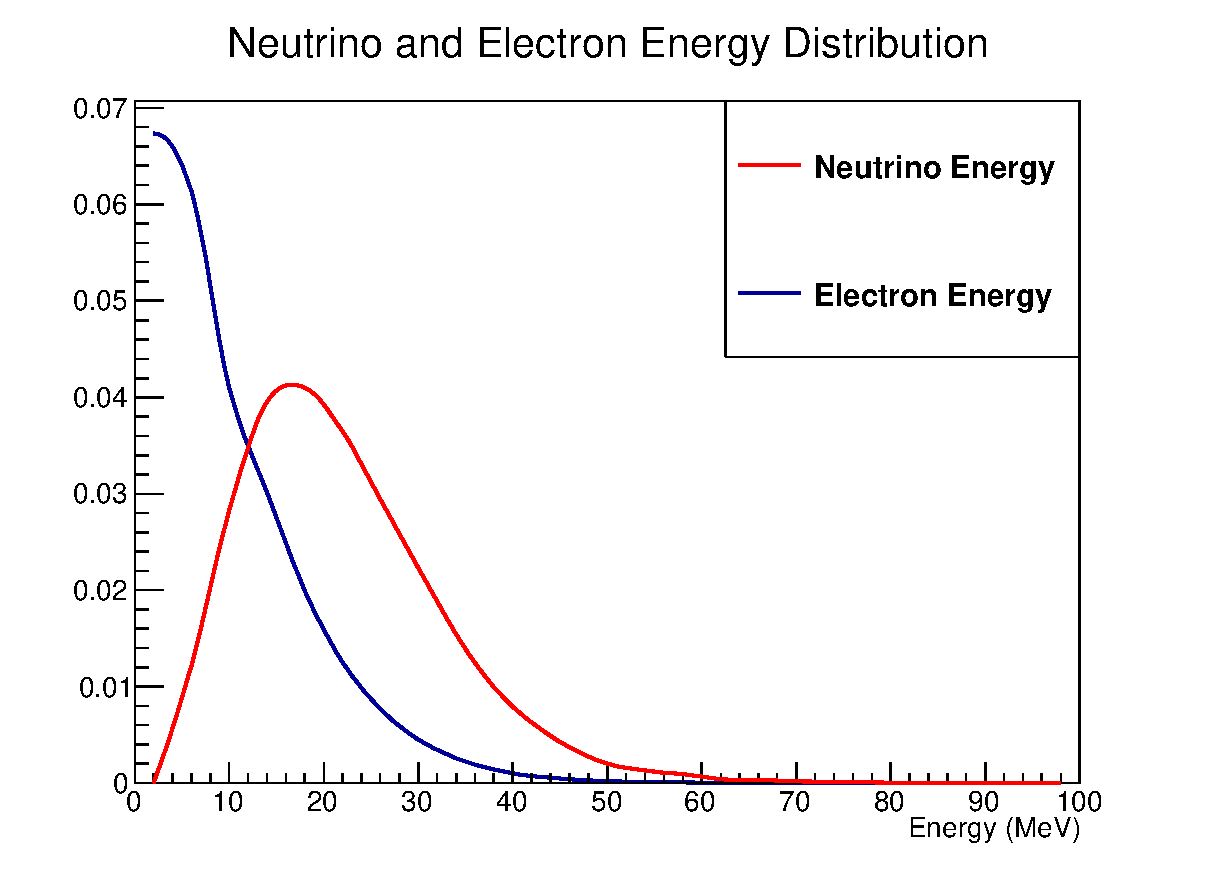
\includegraphics[width=0.75\textwidth]{plots/NuE_energy_dist.eps}
    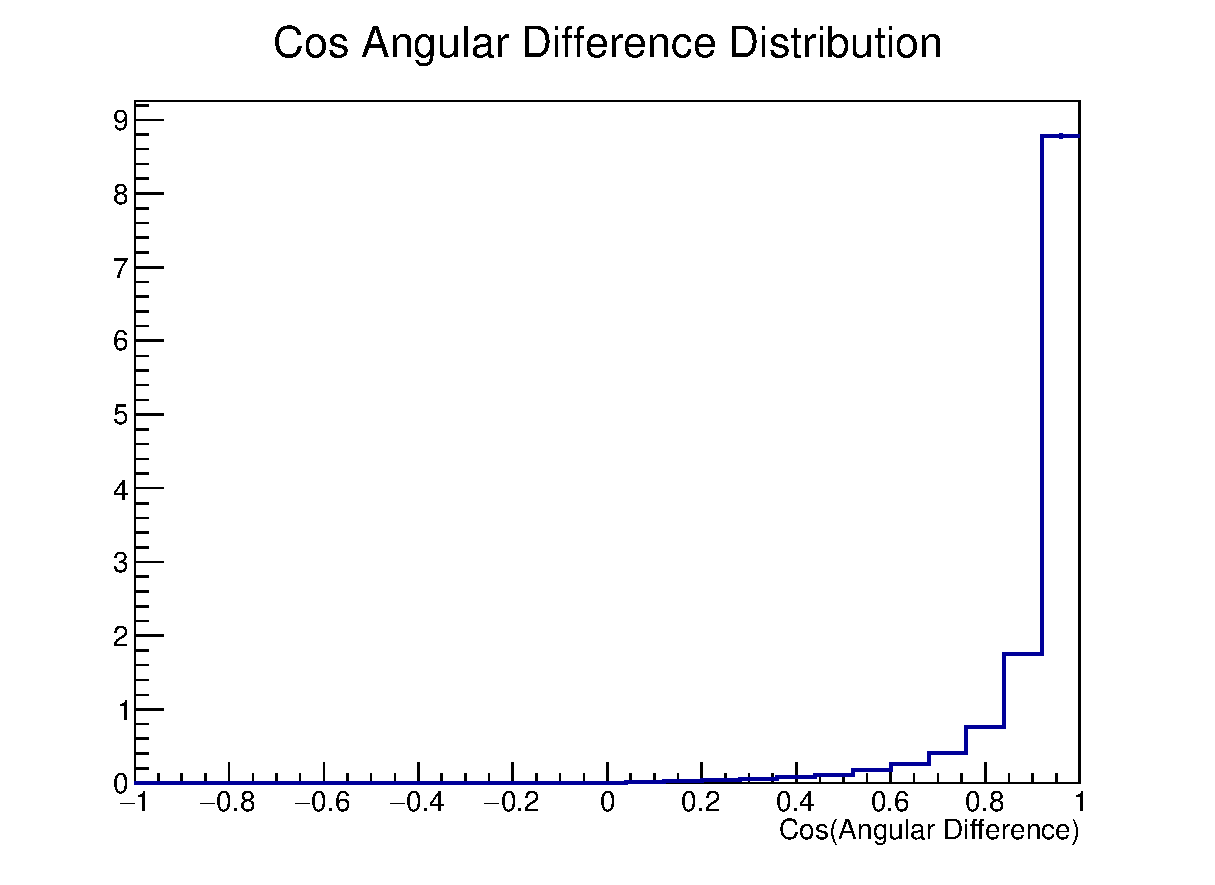
\includegraphics[width=0.75\textwidth]{plots/NuE_angle_dist.eps}
    \caption{Energy and Angular distributions for $\nu$+$e^-$ elastic scattering. Top: Density distribution of the energy of incoming neutrinos (red) and outgoing electrons (blue). Bottom: Density distribution of the cosine of the scattering angle.}
    \label{fig:ES_dist}
\end{figure}

\subsection{Charged Current Interactions}
DUNE is also particularly sensitive to the charged current absorption of $\nu_e$ on $^{40}$Ar: 
\begin{equation}
    \nu_e + ^{40}\text{Ar}\rightarrow e^- + ^{40}\text{K}^*
\end{equation}
The primary observable of this interaction is the $e^-$. The MARLEY generator\cite{gardiner2021simulating} is used to generate the simulated particles for this interaction. The output energy and angular distributions of this interaction are shown in Figures \ref{fig:CC_dist}. 
\begin{figure}[h!]
    \centering
    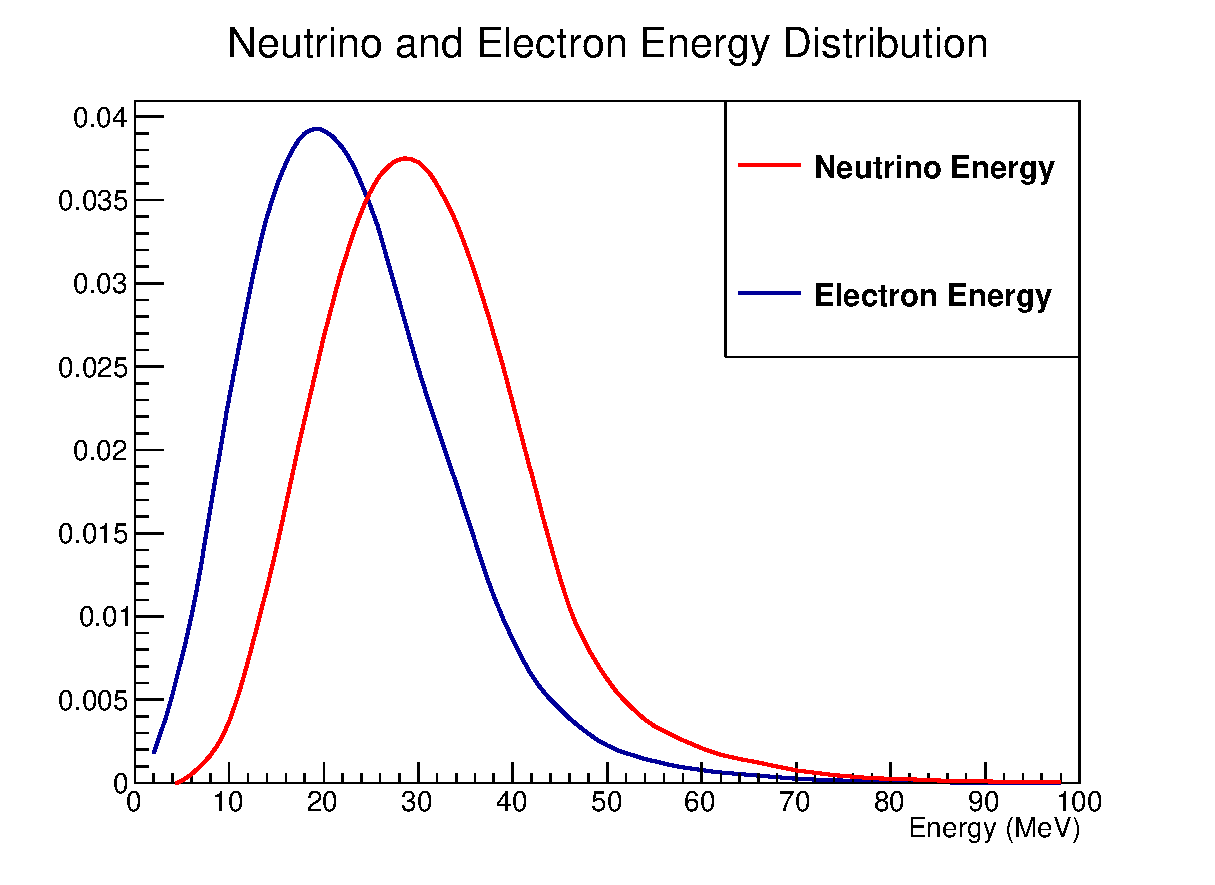
\includegraphics[width=0.75\textwidth]{plots/CC_energy_dist.eps}
    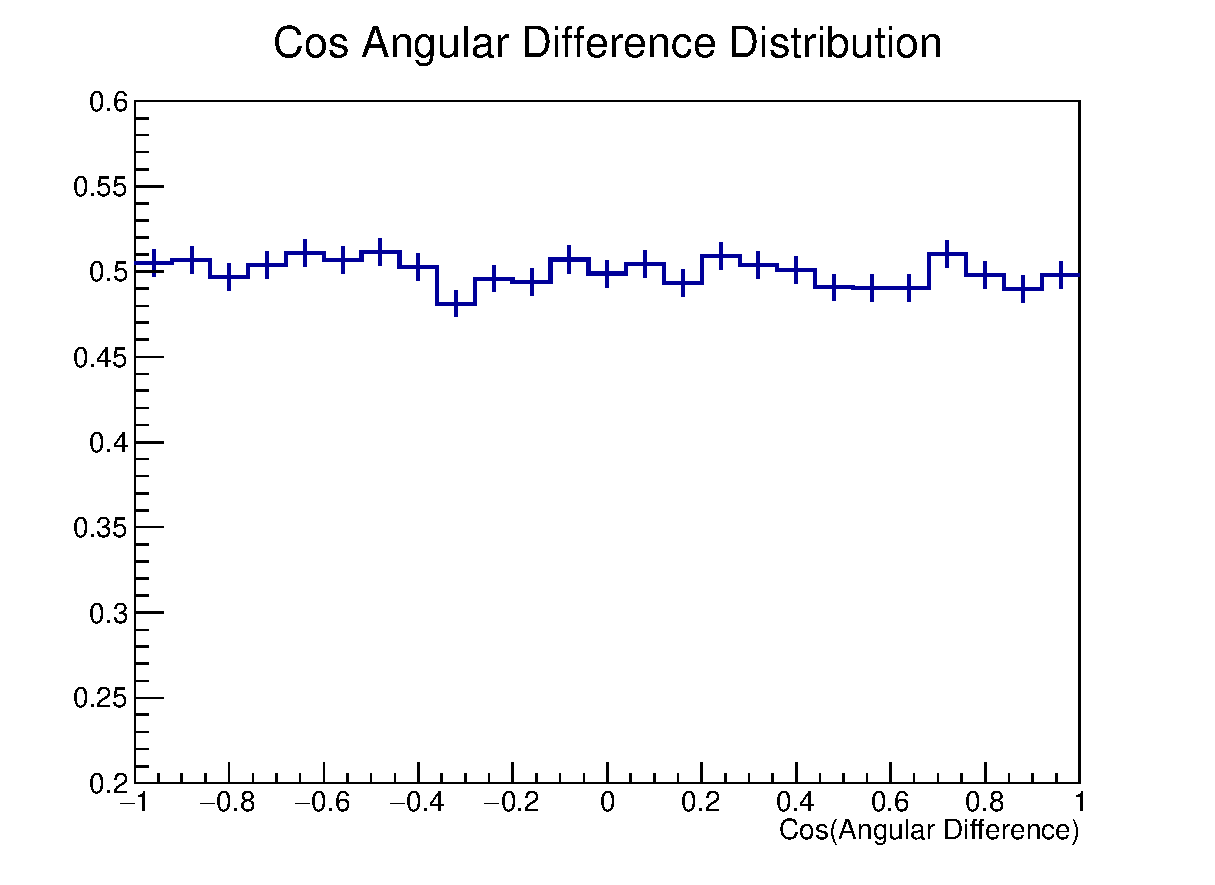
\includegraphics[width=0.75\textwidth]{plots/CC_angle_dist.eps}
    \caption{Energy and Angular distributions for the $\nu_e + \prescript{40}{}{} \text{Ar}$ charged current interaction. Top: Density distribution of the energy of incoming neutrinos (red) and outgoing electrons (blue). Bottom: Density distribution of the cosine of the scattering angle.}
    \label{fig:CC_dist}
\end{figure}
Charged current events are considerably more abundant than the aforementioned elastic scattering events (about 3000 events at 10 kpc for DUNE compared to 300). Yet, the trajectory of the electron does not correlate well with the neutrino direction. This is due to the presence of two (Fermi and Gamow-Teller) competing nuclear matrix elements, $B(F)$ and $B(GT)$. With $B(F)$ correlating with $1 + \frac{v}{c}\cos\theta$ and $B(GT)$ correlating with $1 - \frac{1}{3}\frac{v}{c}\cos\theta$ \cite{gardiner2021nuclear}, these two elements cancel out with each other almost exactly, resulting in a angular distribution that is mostly flat given the event statistics, as shown in the bottom plot of Figure \ref{fig:CC_dist}. Figure \ref{fig:CC_matrix_elements} from \cite{gardiner2021nuclear} shows the contribution of the two matrix elements for a toy SN spectrum. Therefore, the pointing resolution of a supernova depends on a robust classifier between ES and CC events, discussed in a following section.

\begin{figure}
    \centering
    \includegraphics[width=0.55\textwidth]{plots/diff_xsecs_toy-sn3.pdf}
    \caption{The contribution of Fermi and Gamow-Teller matrix elements to the angular distribution for CC events. The two matrix elements cancel out almost exactly in the context of a SN neutrino energy spectrum. Figure is retrieved from \cite{gardiner2021nuclear}.}
    \label{fig:CC_matrix_elements}
\end{figure}


\section{Simulation and Reconstruction Methods}
Full detector Monte Carlo simulations are used to determine the statistical distribution of the considered neutrino events as well as the supernova pointing resolution given the current theoretical models and reconstruction methods. The simulation and reconstruction procedure is carried out with a custom build of DUNE \larsoft \cite{snider2017larsoft} version \texttt{v09\_29\_00}. The custom build features an upgrade to the far detector simulation and reconstruction chain, where upgraded modules from ProtoDUNE studies are incorporated to the far detector workflow. In particular, the upgrade enables more realistic low energy physics simulation, optical detector simulation, and electron drift simulation \cite{rivera}. 

All simulations are done in the \texttt{1x2x6} horizontal drift far detector workspace. The ES and CC event generators are set to generate particles uniformly in the workspace with randomly selected neutrino directions. Standard radiological and detector noise models were used during the simulations. The Projection Matching Algorithm is used for 3D track reconstruction. 

The event display of an example event is shown in Figure \ref{fig:evd_example}. This particular example is an ES event. Near the interaction vertex, there is a cluster of charge depositions. Of note, there is a long track with high charge deposition that corresponds to the primary electron as well as several lower charge short tracks. These tracks may correspond to lower energy final state particles that were produced during the interaction (such as the nuclear remnants of charged current events), or daughter particles of the primary electron created in subsequent interactions. Notably, some daughter particles of the primary electron have directions that correspond to the primary electron, making them useful in determining the starting direction of the primary electron track (discussed later). Additionally, charges may also be registered as a result of radiological decays, such as the decay of $^{39}\text{Ar}$ and electronics noise. These signals occur only for a short period of time compared to the primary electron, are far apart from each other, and are of low amplitude. 
\begin{figure}[h!]
    \centering
    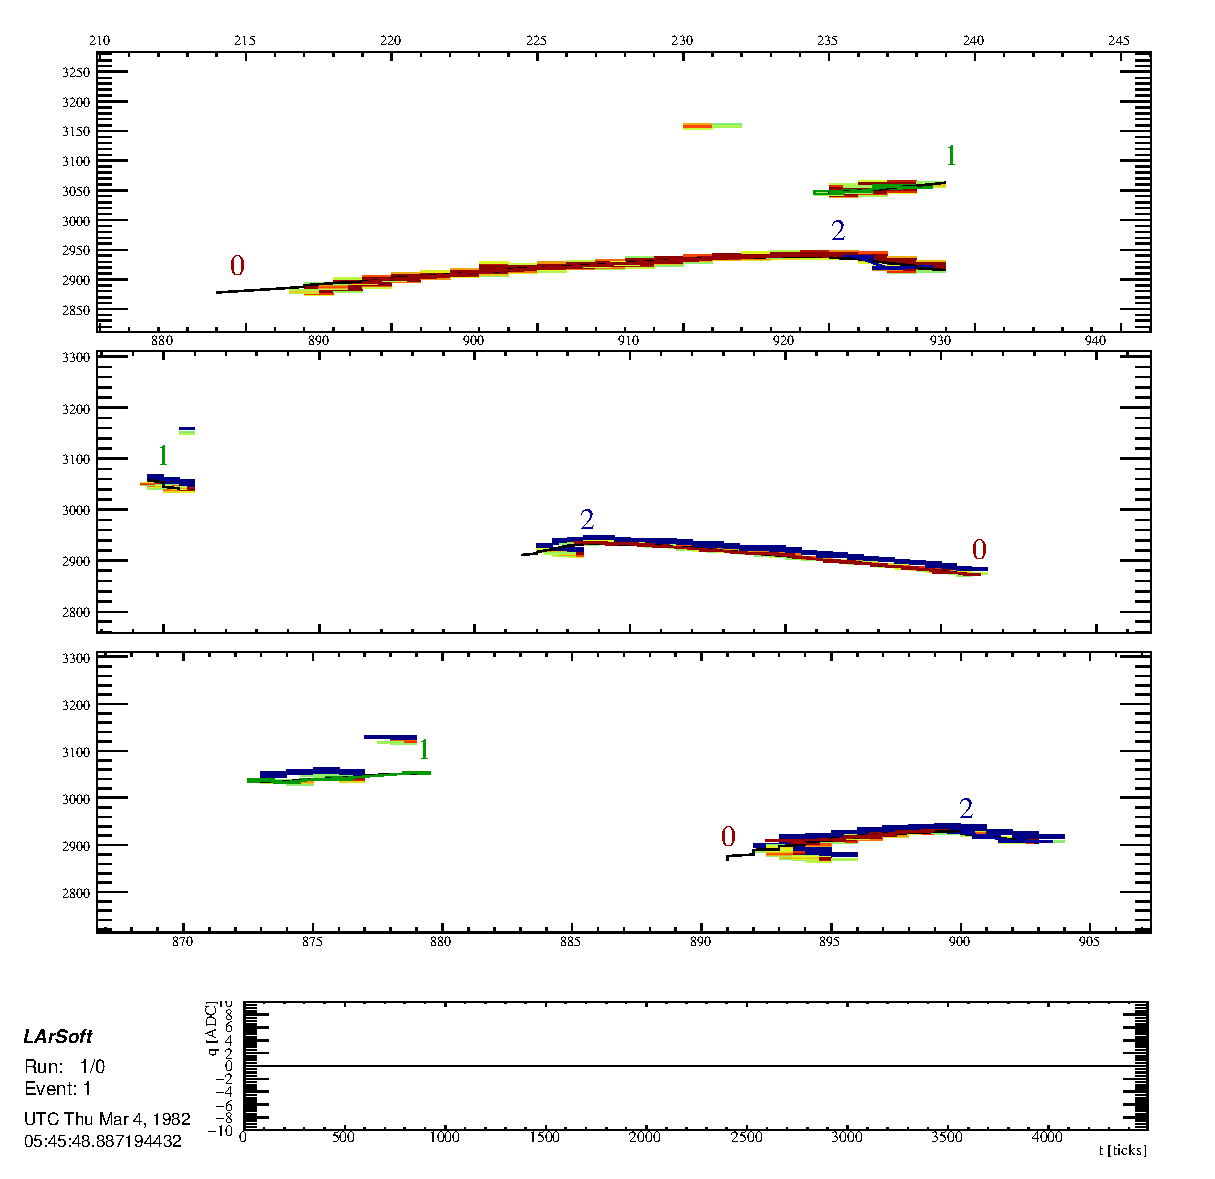
\includegraphics[width=0.75\textwidth]{plots/ES_evd.eps}
    \caption{Example Event Display of an ES Event. The colored square is a heat-map of the charge deposited on each wire segment per time tick. From top to bottom, the three plots show the view of the three wire planes, (U, V, and X respectively) for the Liquid Argon Time Projection Chamber (LArTPC). The trajectories with numerical labels are reconstructed tracks.}
    \label{fig:evd_example}
\end{figure}

The first step in reconstructing the event is to determine the reconstructed track that corresponds to the primary electron. In a noise-free scenario, the track of the primary electron typically has the greatest length, as the electron deposits more charges compared to its daughter particles. However, the presence of radiological decay particles complicate the matter, as a highly energetic radiological decay product may deposit more charge than the primary electron, thus creating a track longer than the primary electron track. Rejection of such scenarios can be done by examining the spatial distance between tracks. Particles associated with the neutrino interactions are closely clustered together, while the radiological particles are sparse and far away from each other. Therefore, radiological tracks are rejected by examining the position of the ten tracks with the highest length and neglecting high-energy tracks that are positioned far away from all other high-energy tracks. 

After the correct track is determined, the electron's direction can then be reconstructed by examining the directional vectors associated with the track. However, there remain ambiguities regarding which side of the track is the start of the track. 3D reconstruction in the DUNE Time Projection Chambers (TPCs) utilizes the timing information to reconstruct the drift coordinate of the event. Therefore, it is not known which side of the track is created first, causing the reconstructed direction to be opposite of the true neutrino direction. This ambiguity is resolved using the adjacent tracks created by daughter particles. The bremsstrahlung gamma rays created by the primary electron create daughter electrons via Compton scattering, the photoelectric effect, and pair production. These daughter electrons thus correlate with the forward direction of the primary electron. The daughter electrons' directions are also expected to correlated with the primary electron's direction more closely when the primary electron is of higher energy. This is confirmed using DUNE Monte Carlo in \cite{roeth2019supernova}. The particular procedure of disambiguating the direction of the primary electron is carried out in a process called ``daughter flipping'', which is also described in \cite{roeth2019supernova}. For each vertex of the selected primary track, the average of the cosines of the angles between the directional vector of the track at the vertex and the unit vector that points from the vertex to each daughter track is calculated. The vertex that has the larger average cosine value is then selected as the starting point of the track.  \cite{roeth2019supernova} also suggests that track selection can potentially be improved by examining the charge deposition along the track, as the particle typically deposits more energy towards the end of its trajectory.

The effect of daughter flipping can be seen in Figure  \ref{fig:daughter_flipping}. The top plot shows that the reconstructed electron directions have a distribution centered around both the parallel and anti-parallel directions with respect to truth, a result of the directional ambiguity of the tracks. By applying daughter flipping, the magnitude of the distribution surrounding the anti-parallel direction is significantly decreased, suggesting that the technique is successful in resolving the ambiguity in track directions. The bottom plot of Figure \ref{fig:daughter_flipping} shows how daughter flipping improves the ``reconstruction resolution'' of the events. ``Reconstruction resolution'' is defined as the angle where 68\% of the events have an angular difference between the true and reconstructed electron direction that is less than that angle. Daughter flipping improves upon the reconstruction resolution of standard reconstruction, particularly at higher electron energies, as there are more daughter tracks when the primary electron energy is high.
\begin{figure}[h!]
    \centering
    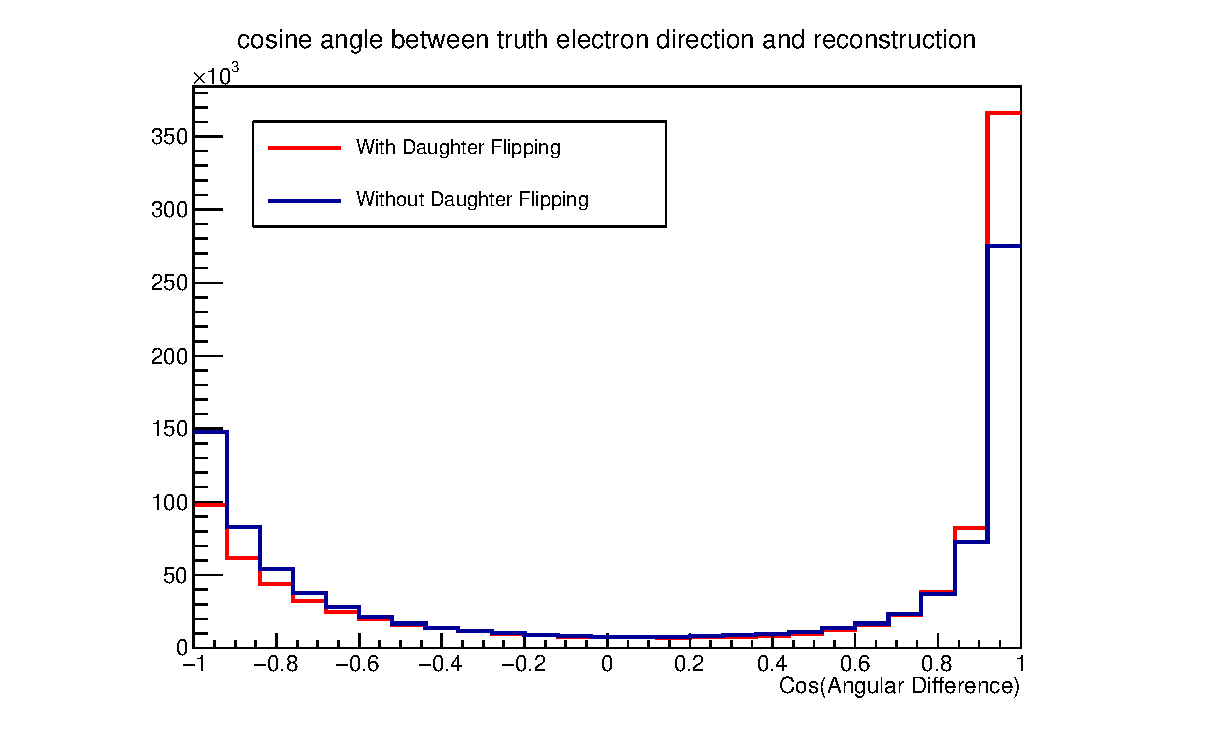
\includegraphics[width=0.75\textwidth]{plots/BiPeak.eps}
    \includegraphics[width=0.75\textwidth]{plots/reco_res_energy.eps}
    \caption{Effectiveness of the daughter flipping algorithm. The top plot shows the bi-modal distribution of the angular difference between true and reconstructed directions, centering around the parallel ($\cos{\theta} = 1$) and anti-parallel ($\cos{\theta} = -1$) directions. Daughter flipping decreases the magnitude of the anti-parallel peak. The bottom plot shows the relationship between the reconstruction resolution (68\% quantile of angular difference) and electron energy. The black curve shows the resolution of perfect track directional disambiguation. Daughter flipping performs better at higher energies, as there are more daughter tracks to reference.}
    \label{fig:daughter_flipping}
\end{figure}

In addition to reconstructing the direction of the electron, the energy of the primary electron is also reconstructed, as the pointing resolution of an event depends on the energy of its electron. The reconstruction is done by summing the total charge deposited near the interaction vertex (with a distance cut applied at 5 times the radiation length of Ar), and mapping charge to energy using a linear relationship (shown in Figure \ref{fig:chargeenergy}). The distance cut is applied to reject the contribution of radiological particles far away from the interaction vertex. Charge loss due to drift is also considered and corrected for using optical detector timing information. 
\begin{figure}
    \centering
    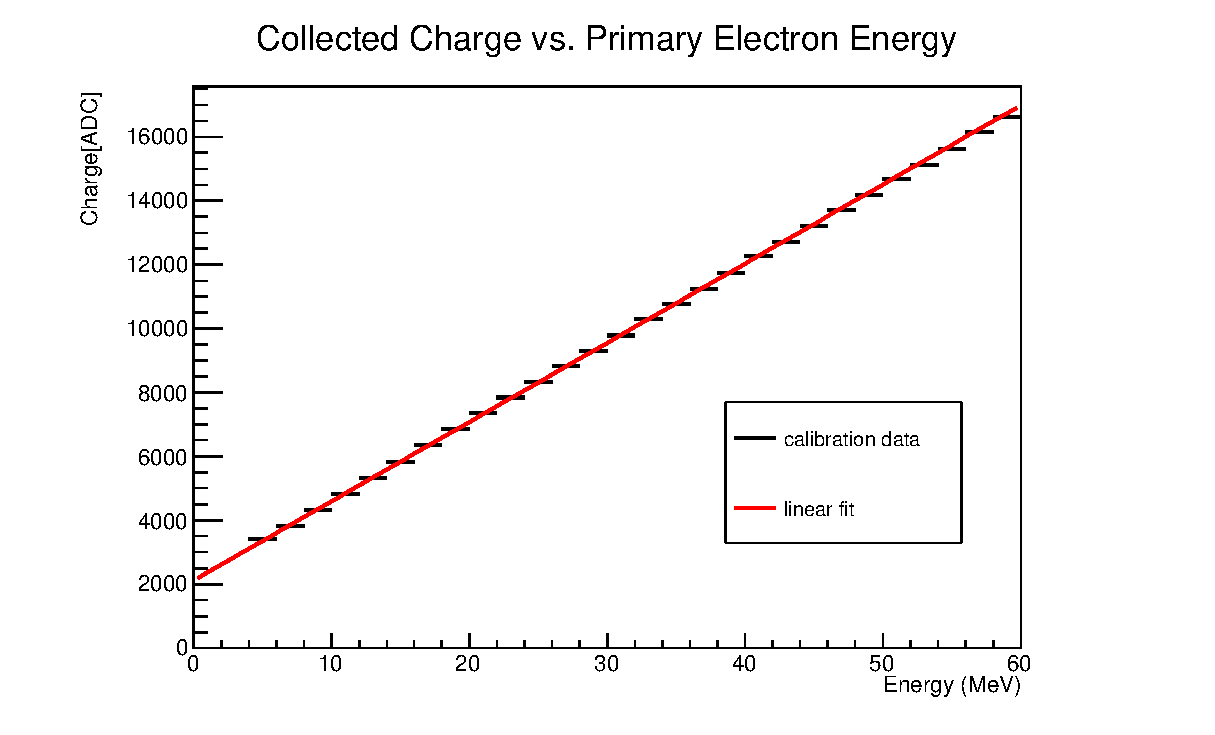
\includegraphics[width=0.75\textwidth]{plots/ChargeEnergy.eps}
    \caption{Linear relationship between collected charge and electron energy.}
    \label{fig:chargeenergy}
\end{figure}

\section{Reconstructing Supernova Direction}
The reconstructed information for each individual neutrino event is combined to reconstruct the direction of a supernova using a maximum likelihood method. For an event with known interaction type, the probability density function (PDF) has the functional form of $p_{r}(E_i, \hat{d}_i; \hat{d}_{SN})$, where the index $r$ indicates the neutrino channel: ES or CC. $E_i$ and $\hat{d}_i$ are the reconstructed energy and direction of the specific event, and $\hat{d}_{SN}$ is the direction of the supernova. The PDF is a function of the reconstructed energy as well as the inner product of the supernova direction and reconstructed electron direction, $\hat{d}_i \cdot  \hat{d}_{SN} = \cos{\theta_{SN}}$. The PDFs are determined using \larsoft simulation of 1M events in each channel. The Monte Carlo samples are divided into energy bins, spanning from 0 to 40 MeV with a width of 2 MeV per bin, and from 40 MeV to 70 MeV (plus an overflow bin) at 10 MeV per bin. For a given energy value, the closest bin value is used as the output value.

The generated PDFs are shown in Figure \ref{fig:2dpdfs} for both ES and CC events. For the CC channel, the low correlation between electron and neutrino directions render the PDF mostly flat. ES interactions demonstrate high correlation between supernova direction and reconstruction direction. A bi-modal distribution is still seen due to the tracks' directional ambiguity, but the true peak (centering around $\cos{\theta_{SN}} = 1$) has much higher amplitude than the peak around the flipped direction ($\cos{\theta_{SN}} = -1$). In particular, at higher electron energy, the pointing of ES events improves both in variance around the supernova direction, as well as in track directional disambiguation. The improved performance at high energy is further demonstrated in the 10 MeV energy slices of the ES PDF shown in Figure \ref{fig:pdf_slices}.

\begin{figure}[h!]
    \centering
    \includegraphics[width=0.6\textwidth]{plots/ES_pdf/ES_pdf_2d.eps}
    \includegraphics[width=0.6\textwidth]{plots/CC_pdf/CC_pdf_2d.eps}
    \caption{Probability density functions of ES and CC events. The ES PDF demonstrates high correlation between supernova and electron directions. The CC PDF is mostly flat, as the correlation between electron and neutrino direction is weak.}
    \label{fig:2dpdfs}
\end{figure}

\begin{figure}[h!]
    \centering
    \subfigure[]{\includegraphics[width=0.48\textwidth]{plots/ES_pdf/0-10.eps}}
    \subfigure[]{\includegraphics[width=0.48\textwidth]{plots/ES_pdf/20-30.eps}}
    \subfigure[]{\includegraphics[width=0.48\textwidth]{plots/ES_pdf/40-50.eps}}
    \subfigure[]{\includegraphics[width=0.48\textwidth]{plots/ES_pdf/60-70.eps}}
    \caption{Several bins for the PDF of the ES interaction, re-binned to 10 MeV / bin. The relative magnitude of the peak surrounding $\cos{\theta_{SN}} = 1$ (the parallel direction) increases as energy increases because daughter flipping improves at high energies. The widths of the peaks also decrease, indicating a decrease in directional variance.}
    \label{fig:pdf_slices}
\end{figure}

Using the determined PDFs, supernova direction can then be reconstructed using the maximum likelihood method. Specifically, given a set of reconstructed events, likelihood as a function of supernova direction can be expressed as:
\begin{equation}
    \mathcal{L}(\hat{d}_{SN}) = \prod_i p(E_i, \hat{d}_i; \hat{d}_{SN})
    \label{eq:likelihood}
\end{equation}

assuming perfect classification between ES and CC events, $p = p_{ES}$. The effect of imperfect classifications is discussed later.

Maximizing $\mathcal{L}$ is equivalent to minimizing the negative logarithm of $\mathcal{L}$:
\begin{equation}
    \begin{split}
        - \log \mathcal{L}(\hat{d}_{SN}) &= - \log \qty[\prod_i p(E_i, \hat{d}_i; \hat{d}_{SN})]\\
        &= - \sum_i \log p(E_i, \hat{d}_i; \hat{d}_{SN})
    \end{split}
    \label{eq:neglog}
\end{equation}
By parameterizing $\hat{d}_{SN}$ using the azimuth and zenith angles, the supernova direction can then be reconstructed by solving a two-variable minimization problem. The minimization is done using a grid search. The grid search also outputs the likelihood function value for all directions, which can be filled into a HEALPix \cite{gorski2005healpix} sky map. An example output of this reconstruction procedure is shown in Figure \ref{fig:skymap}, which shows that the likelihood function typically has two local minima that are 180 degrees away from each other. This is a result of the remaining ambiguity in track direction.

\begin{figure}[h]
    \centering
    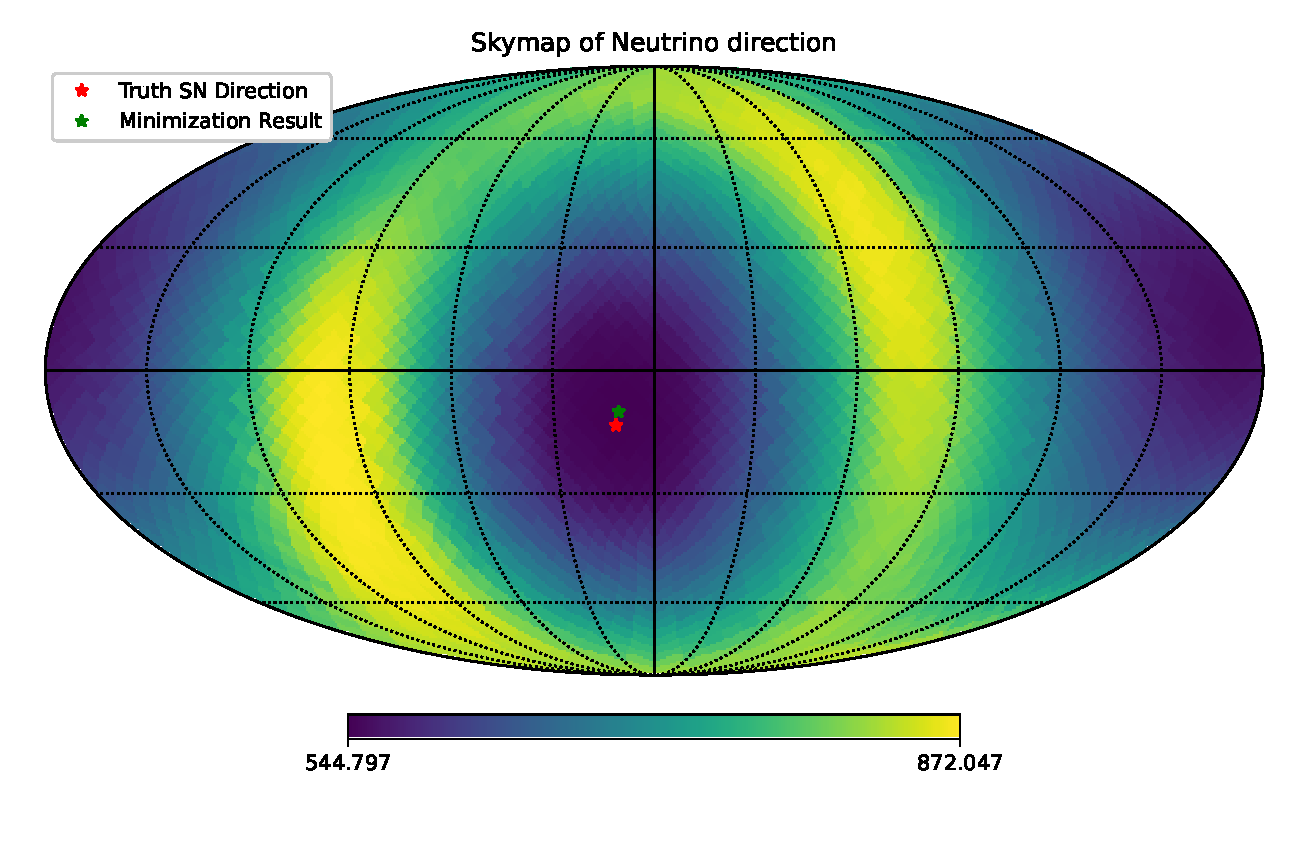
\includegraphics[width=0.9\textwidth]{plots/skymap.eps}
    \caption{An example sky map filled with the negative log likelihood values. Reconstruction is done purely based on ES events, with no mixed-in CC events.}
    \label{fig:skymap}
\end{figure}

\section{Performance}
Supernova bursts are synthesized to evaluate the performance of the reconstruction algorithm. Simulation is done by randomly picking ES and CC events from a large pool of events with uniformly distributed neutrino directions. The number of events selected per burst is based on the expected number of interactions for a 10 kpc supernova, as calculated by \snowglobes. For each selected event, the reconstructed direction is then rotated such that all events correspond to the same neutrino direction. One thousand supernova bursts are simulated and reconstructed using only ES events, and a pointing resolution of around 3.7 degrees is achieved. ``Pointing resolution'' is defined as the angle under which 68\% of the truth-reconstruction angular difference of the supernova burst samples lie. The distribution of the truth-reconstruction angular difference is shown in Figure \ref{fig:pointres}. It is also worth noting that one of the simulated bursts' reconstructed direction was more than 90 degrees away from the supernova position. The reconstructed direction of this event is very close to being anti-parallel to the supernova direction, suggesting that it landed in the incorrect local minimum. In practice, the certainty of a likelihood function in selecting one of the two opposite directions can be quantified by examining the difference between the likelihood function values at the two minima. For the singular burst that had a flipped reconstruction direction, the difference of the two minima was around $10^{-4}$, where the next smallest difference was greater than 1. 

\begin{figure}
    \centering
    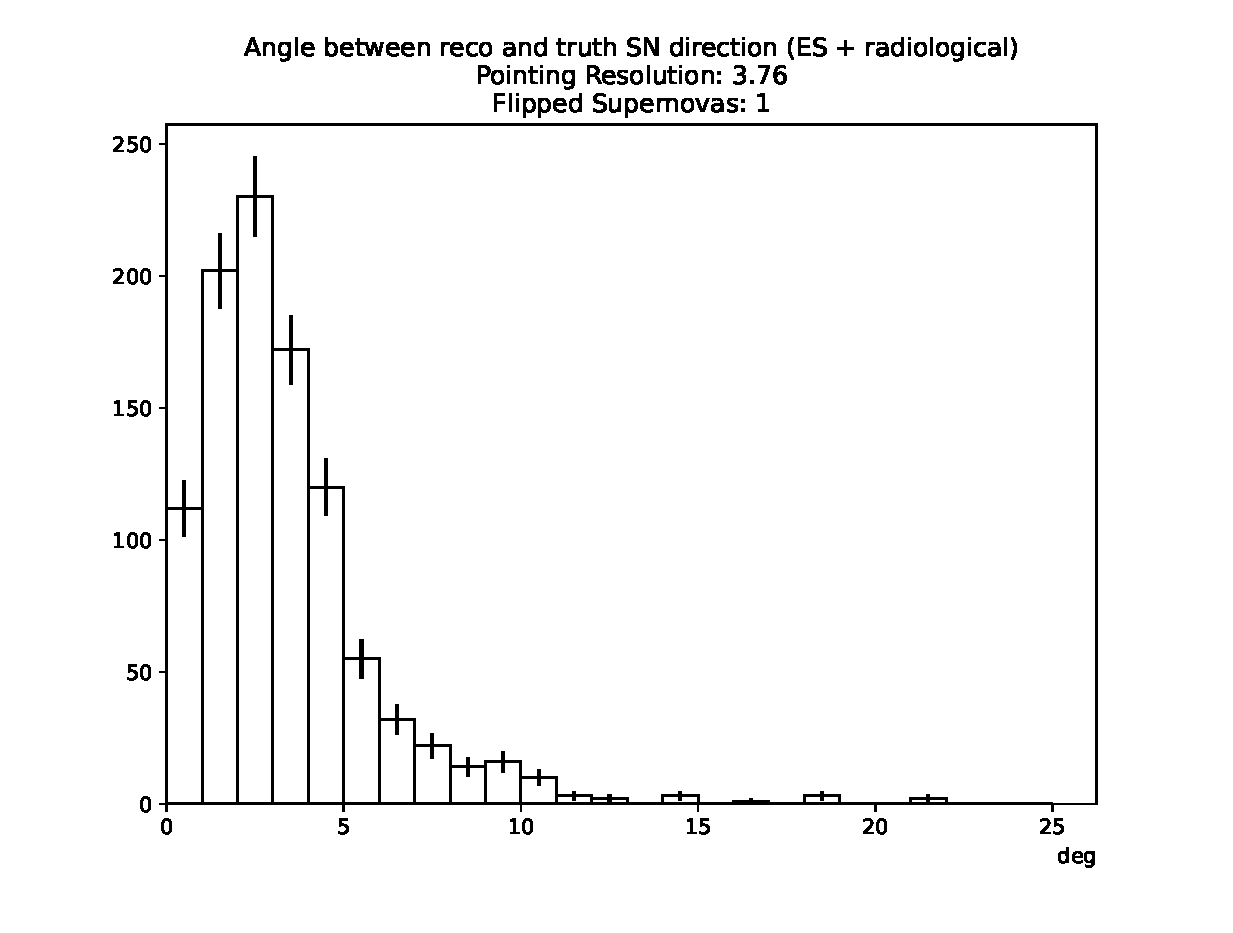
\includegraphics[width=0.75\textwidth]{plots/pointres.eps}
    \caption{Distribution of the angular difference between the reconstructed and true supernova direction, for 1000 simulated supernova bursts. The singular event with the flipped reconstruction is excluded from the plot.}
    \label{fig:pointres}
\end{figure}

While the pointing resolution using only ES events promises good pointing performance, this is not the complete picture, as it is difficult in practice to distinguish between ES and CC events. The quality of a realistic classifier can be quantified in the form of a confusion matrix:
\begin{equation}
    C = \begin{bmatrix}c_{ES\rightarrow ES} & c_{ES\rightarrow CC}\\c_{CC\rightarrow ES} & c_{CC\rightarrow CC}\end{bmatrix}
\end{equation}

The elements of this matrix are expressed in the form of $c_{A\rightarrow B}$, which describes the portion of events of interaction type $A$ that are classified as interaction type $B$. This confusion matrix is normalized to be independent of the expected number of events for each interaction. Assuming no loss of events due to detector inefficiency, the rows of the matrix will sum to one. Furthermore, the worst-case scenario of reasonable classifier can be represented by a confusion matrix with all of its elements being $1/2$, which effectively represent a completely random grouping of all events into two groups.

In adopting a realistic classifier, the aforementioned reconstruction procedure is effectively unchanged, except for that the PDF $p$ used in (\ref{eq:likelihood}) and (\ref{eq:neglog}) is no longer $p_{ES}$, but a sum of $p_{ES}$ and $p_{CC}$, weighted by the expected number of events from each interaction in the classification channel. As useful pointing information is only present in ES events, only the ES classification channel is used for direction reconstruction. Subsequently, the only elements in the confusion matrix $C$ that effects the pointing effect is $c_{ES\rightarrow ES}$ and $c_{CC\rightarrow ES}$. Figure \ref{fig:mixing} shows a map of pointing resolution as a function of the two relevant matrix elements. At the realistic worst-case scenario (where both elements are equal to $0.5$), the pointing resolution is $102$ degrees. While robust classifiers can yield highly accurate pointing results, even a weak classifier can yield  quite useful pointing resolution. At $c_{ES\rightarrow ES} = 0.6$, only 20\% better than random selection, the pointing resolution can reach around 40 degrees, significant enough to determine the quadrant of the sky that the supernova belongs to. An optimistic estimate of a boosted decision-tree based classifier is established in \cite{erin_conley_2020_4122909} at $c_{ES\rightarrow ES} = 0.86$ and $c_{ES\rightarrow ES} = 0.040$. With this classifier, the pointing resolution is at $5.3$ degrees. However, no noise was simulated in this study, meaning that the quality of the classifier is likely overly optimistic. 



\begin{figure}
    \centering
    \includegraphics[width=0.75\textwidth]{plots/mixing.eps}
    \caption{Pointing resolution as a function of ES true positives ($c_{ES\rightarrow ES}$) and CC false negatives ($c_{CC\rightarrow ES}$). For each pair of values, 100 supernova events are simulated to determine the pointing resolution. }
    \label{fig:mixing}
\end{figure}

\section{Summary}
A framework to reconstruct supernova direction at DUNE is described. By reconstructing the ES and CC events during a supernova burst, the supernova direction can be reconstructed using the direction between the supernova neutrino and the outgoing electron. Monte Carlo simulations are used to determine the pointing resolution of this framework. With perfect event classification, the pointing resolution is 3.7 degrees for 68\% of the events for supernovae at a distance of 10 kpc. Considering classification errors in realistic event classifiers, an optimistic estimate of the pointing resolution is at 5.3 degrees with 68\% coverage.


%----BIBLIOGRAPHY

\clearpage
\bibliographystyle{unsrt}
\nocite{*}
\bibliography{mybib}
\end{document}
